\documentclass[11pt]{article}
 \usepackage[margin=1in]{geometry} 
\usepackage{amsmath,amsthm,amssymb,amsfonts}
\usepackage{enumerate}
\usepackage{color}
\usepackage{mathtools}
\usepackage{pgfplots}
\usetikzlibrary{quotes,angles}
\pgfplotsset{compat=newest}

\usepackage{hyperref}
\hypersetup{
    colorlinks=true,
    linkcolor=black,
    filecolor=blue,      
    urlcolor=blue,
}
 
\newcommand{\N}{\mathbb{N}}
\newcommand{\Z}{\mathbb{Z}}
\newcommand{\C}{\mathbb{C}}
\newcommand{\Q}{\mathbb{Q}}
\newcommand{\R}{\mathbb{R}}
\newcommand{\plot}{\begin{tikzpicture}}
\newcommand{\eplot}{\end{tikzpicture}}
\newcommand{\p}{\begin{problem}}
\newcommand{\epr}{\end{problem}}
\renewcommand{\vec}[1]{\mathbf{#1}}
\renewcommand{\tilde}[1]{\expandafter\hat{#1}}
\newcommand{\mat}[1]{\mathbf{#1}}


\newenvironment{problem}[2][Problem]{\begin{trivlist}
\item[\hskip \labelsep {\bfseries #1}\hskip \labelsep {\bfseries #2.}]}{\end{trivlist}}
%If you want to title your bold things something different just make another thing exactly like this but replace "problem" with the name of the thing you want, like theorem or lemma or whatever
 
\begin{document}
 
%\renewcommand{\qedsymbol}{\filledbox}
%Good resources for looking up how to do stuff:
%Binary operators: http://www.access2science.com/latex/Binary.html
%General help: http://en.wikibooks.org/wiki/LaTeX/Mathematics
%Or just google stuff
 
\title{SafeFlight}
\author{Martin Deegan}
\maketitle

\tableofcontents

\section{Introduction}

SafeFlight is a quadcopter flight controller written entirely in Rust. It runs on a Raspberry Pi 3 Model B and features everything from low level sensor readings and management up to high level state estimation and flight control.

SafeFlight started in the Summer of 2017 as a personal project and continued as a side project during school. This is my first dabble into robotics and increased my interest in robotics profoundly.

This document is a contains all of the mathematics and concepts that have gone into SafeFlight's subsystems and will be updated as more is added. Hopefully, this will act as a guide to some people looking to work on their own robotics projects and will simplify many of the confusing topics presented on the internet.

\section{Extended Kalman Filter}
SafeFlight uses an Extended Kalman Filter for attitude estimation and position estimation. There is a 20-dimensional state that measures position (North, East, Down), velocity (NED), orientation, gyroscope bias, accelerometer bias, magnetic field, and sea level pressure. We denote the state as $\vec{x}$ and the error state as $\delta \vec{x}$.

$$\vec{x} = \begin{bmatrix}
p\\ v\\ q\\ b_g\\ b_a\\ m\\ b
\end{bmatrix}~~~~ \vec{\delta x} = \begin{bmatrix}
\delta p\\
\delta v\\
\delta \theta\\
\delta b_g\\
\delta b_a\\
\delta m \\
\delta b
\end{bmatrix}$$

Much of the derivation of the prediction step in Kalman Filter comes from the work of Joan Sola in this \href{http://www.iri.upc.edu/people/jsola/JoanSola/objectes/notes/kinematics.pdf}{paper}.
\subsection{How does the Extended Kalman Filter work?}
The EKF is an amazing tool for combining any number of sensor readings into one big estimation system. It works by tracking both your predicted state, $\vec{x}$, and your uncertainty, $\mat{P}$, which is represented as a covariance matrix (how much each value varies with respect to each other). By tracking your uncertainty, you can accuratly update your state when you receive an absolute measurement (that is usually noisy). Here I will explain the two parts of a Kalman Filter.
\subsubsection{Prediction}
	Often you will have high frequency measurements from your array of sensors that will be quite accurate. Examples are a gyroscope or an accelerometer. These measurements will be enough to predict your state for a few seconds, but will drift away from the true value over time.
	
Some notation quickly: $\vec{x}$ is the state (position, velocity, etc...) and $\vec{u}$ is a control variable (gyroscope readings, accelerometer readings, etc...). This control variable contains high frequency measurements. We can define a function (usually nonlinear) to represent how our state changes now that we have new readings. In the quadcopter case, this function is definitely nonlinear due to the rotation.

$$f(\vec{x}_{k-1}, \vec{u}) = \vec{\tilde{x}}_k$$

Where $\vec{\tilde{x}}_k$ is the predicted state. In a prediction step you usually integrate something. For example you can integrate angular velocity to get orientation or you can integrate acceleration to get velocity. Example:

$$\vec{v}_{k} = \vec{v}_{k-1} + \vec{a}_k\Delta t$$

How do we track uncertainty? Just as each part of the state has an transition function attached to it, the error state also follows the same transition function. Example:
$$\vec{\delta v}_k = \vec{\delta v}_{k-1} + \vec{\sigma}_a\Delta t$$
Where $\vec{\sigma_a}$ is the variance (noise) of the accelerometer. There is one slight difference, we don't know the error state, we only know how uncertain we are. If we knew the error state, we could simply subtract it and we would know exactly where we are! So instead, we can transition our uncertainty.

This is where the EKF gets its "Extended" name. We need to transition our covariance matrix $\mat{P}$ somehow in the same way we transition $\vec{x}_{k-1}$ to $\vec{\tilde{x}}_k$ with $f$. In a normal Kalman Filter $f$ is represented as a linear transformation (a matrix), however here it is a nonlinear function. To do this we need to linearize $f$ somehow. If you remember Taylor expansions form calculus, you have the single variable case:
$$f(x_k) = f(x_{k-1}) + f'(x_{k-1})(x-a) + \frac{f''(x_{k-1})}{2!}(x-a)^2 + \frac{f'''(x_{k-1})}{3!}(x-a)^3 + \dots$$

This is very similar to our transition function. In fact, we can represent the change in our state as a tiny little step in the direction of the derivative. This is simply a first order multivariable Taylor series where our change is just the change in time:
$$f(\vec{x}_{k-1}, \vec{u}) = \vec{x}_{k-1} \oplus \vec{\delta_{predicted}} \approx \vec{x}_{k-1} \oplus \frac{\partial f(\vec{x}_{k-1})}{\partial \vec{x}}\Delta t$$


Where $\oplus$ represents a small addition to the state and $\vec{\delta_{predicted}}$ is that small change amount. In our case, we have a multivariable function so the derivative is a jacobian in which case we can use the multivariable Taylor Series. Here is an example of a first order multivariate Taylor Series:
$$f: \R^n \to \R^m$$
$$f(\vec{x}) = f(\vec{x}_0) + \frac{\partial f_1(\vec{x}_0)}{\partial x_1}(x_1 - a_1) + \dots + \frac{\partial f_1(\vec{x}_0)}{\partial x_n}(x_n - a_n) + \dots $$ 
$$+ \frac{\partial f_m(\vec{x_0})}{\partial x_1}(x_1 - a_1) + \dots + \frac{\partial f_m(\vec{x}_0)}{\partial x_n}(x_n - a_n)$$
$$= f(\vec{x}_0) + \frac{\partial f}{\partial \vec{x}}(\vec{x}- \vec{a}) = f(\vec{x}_0) + \mat{J}(f)(\vec{x}-\vec{a})$$
So we get $\mat{F} = \left.\frac{\partial f}{\partial \vec{x}}\right|_{\vec{x}_{k-1}}$ is the jacobian of $f$ evaluated at $\vec{x}_{k-1}$. $\mat{F}$ is the linearized version of $f$ and we can now update the covariance matrix by using the following identity:
$$\mat{P}_{k} = \mat{F} \mat{P}_{k-1} \mat{F}^T$$
This idenetity basically says "if you act on these variables ($\vec{x}$) with this function $\mat{F}$, then their covariances will update in this way." This only transfers existing uncertainties. At each step we add more uncertainty with each reading. We can represent these uncertainties with a diagonal matrix $\mat{Q}$ where each component is the variance (noise) corresponding to each of the values in the control vector $\vec{u}$. We now need to know how to update $x_p$ based on these new noises so we need to take another jacobian.
$\mat{L} = \left.\frac{\partial f}{\partial \vec{u}}\right|_{\vec{x}_{k-1}}$. Then we can use similar reasoning as above to get:
$$\mat{P_k} = \mat{F} \mat{P}_{k-1} \mat{F}^T + \mat{L} \mat{Q} \mat{L}^T$$

This is our completed prediction step.
\subsubsection{Update}
The update step works a little differently, but has many of the same concepts as above. As I said above, the prediction measurements tend to drift over time so we need some way to keep them in check. Update measurements are usually slow and noisy, but give us an absolute reading with respect to the state. For example: our prediction could use the accelerometer to track position over time, but will eventually have too much error to be worth using. Adding a GPS would correct our position errors and reassure us of where we are. 

Note that there is no way to reduce uncertainty with the prediction step so the update step is crucial to have any sense of where you are. If we have multiple "update" sensors, we will  run an update step for each one individually.\\

Suppose we have a sensor that gives us some reading in the form of a vector 
$$\vec{z}_m = \vec{z}_t + \vec{w}$$
Whatever this sensor is measuring, we know it is an absolute measurement meaning it is near the correct value of whatever it is measuring, $\vec{z}_t$, with some extra noise, $\vec{w}$.

We need a way to "expose" our error state. Remember, we don't know it, we just know how uncertain we are. So we create some function (usually nonlinear) that takes our state (predicted) and outputs a measurement in the exact same format as the sensor measurement.
$$h(\vec{\tilde{x}}_k) = \vec{z}_p$$
Note that if we let $\vec{x}_t$ be the absolute true state, then $$\vec{z}_m = h(\vec{x}_t) + \vec{w}$$
So now we have a way of exposing our error. First we take the residual $\vec{z} = \vec{z}_m - \vec{z}_p$. $\vec{z}$ represents the error in our state. We just need a way to convert it into the form $\delta \vec{x}$ so we can remove that error from our predicted state $\tilde{\vec{x}}_k$ to get the optimal state $\vec{x}_k$. Just like in the prediction step we updated the uncertainty by using the transition function on it, now we do something very similar, we convert this residual into the error state using the same function we used to create it, $h$. First, we need to linearize it though.
$$\mat{H} = \left.\frac{\partial h}{\partial \vec{x}}\right|_{\tilde{\vec{x}}_k}$$
Also define $\mat{R}$ as the variance (noise) of the update sensor in a diagonal matrix. We can measure how much the noises affect the measurement too:
$$\mat{M} = \left.\frac{\partial h}{\partial \vec{z}}\right|_{\tilde{\vec{x}}_k}$$
So in total, the uncertainty of the whole state after the update can be put as
$$ \mat{S} = \mat{H} \mat{P}_k \mat{H}^T + \mat{M} \mat{R} \mat{M}^T$$
So we have the uncertainty from the prediction step $\mat{P}$ and the uncertainty from the update step $\mat{S}$. We use the uncertainty to decide how much to trust the prediction or how much to trust the update measurement. We do this by computing the Kalman gain.\\
$$\mat{K} = \mat{P}_k \mat{H}^T \mat{S}^{-1}$$
Then we compute the error state.
$$\vec{\delta x}_k = \mat{K} \vec{z}$$
Now we have "exposed" the error in our system and we can remove that error.
$$\vec{x}_k = \vec{\tilde{x}}_k \oplus \vec{\delta x}_k$$
And we reset the uncertainty after we updated (became more certain). Here the $\oplus$ represents some way of adding the error state into our state. Most of the time it will be addition, but for example, quaternions do not simply add together.

Finally, we reset the covariance matrix after decreasing our uncertainty.
$$\mat{P}_k  = (\mat{I} -\mat{KH})\mat{P}_k(\mat{I}-\mat{KH})^T + \mat{KRK}^T$$

A bit more about the different matrices. $\mat{H}$ and $\mat{K}$ are very  closely related. $\mat{H}$ serves as a linearized transition function betweem the error state to the measurement vector. $\mat{K}$ is the opposite, it takes an measurement error $\vec{z}$ and converts it into an error state vector. Since these functions are defined by jacobians, the error state propagates properly even though measurement error may have a vastly different dimension than the  state error.
$$\mat{K} \in \R^{m\times n} ~~ \mat{H} \in \R^{n \times m}$$
The errors:
$$\vec{\delta x} \in \R^m ~~ \vec{z} \in \R^n$$
\subsection{Quaternion Error State}
SafeFlight represents the orientation as a quaternion. This means we have 4 variables to represent 3 degrees of freedom. As a result, the error state can reach singularities by using a 4 vector as a quaternion error.

Instead we use $\vec{\delta \theta}$ defined in the following way.
$$\vec{q} = \begin{bmatrix}
\sin \theta~ \vec{v}\\
\cos \theta
\end{bmatrix} = \begin{bmatrix}
\frac{1}{2}\delta \vec{\theta}\\
1
\end{bmatrix}$$

Since $\vec{\delta q}$ is small, $\cos\theta \approx 1$ and therefore, we can use this approximation. Because of this, our error state is smaller than our main state. This messes up our jacobians because now we have a covariance in $\R^{19\times 19}$, but we are taking jacobians with respect to our 20 dimensional state vector. To fix this we need to take our jacobians with respect to our error state. Example:
$$\mat{F} = \frac{\partial f}{\partial \delta \vec{x}} = \frac{\partial f}{\partial \vec{x}}\frac{\partial \vec{x}}{\partial \delta \vec{x}}$$
Using the chain rule, we can get jacobians with respect to our error state.
$$\mat{D} = \frac{\partial \vec{x}}{\partial \delta \vec{x}} = J(\vec{x} \oplus \delta \vec{x})$$
However you define your error state addition, you need its jacobian to update your error state properly. So for all jacobians defined in this document, you will need to multiply by $\frac{\partial \vec{x}}{\partial \delta \vec{x}}$ to get it in the correct form (only if using quaternions).

Using JPL styled quaternions, you will get this jacobian. 

$$\frac{\partial \vec{x} \oplus \delta \vec{x}}{\partial \delta \vec{x}} = \begin{bmatrix}
\frac{\partial \vec{p+\delta p}}{\partial \delta \vec{p}}\\
& \frac{\partial \vec{v+\delta p}}{\partial \delta \vec{v}} \\
& & \frac{\partial \vec{q \otimes \delta q}}{\partial \delta \vec{\theta}}\\
& & & \frac{\partial \vec{b_g+\delta b_g}}{\partial \delta \vec{b_g}}\\
& & & & \frac{\partial \vec{b_a+\delta b_a}}{\partial \delta \vec{b_a}}\\
& & & & & \frac{\partial \vec{m+\delta m}}{\partial \delta \vec{m}}\\
& & & & & & \frac{\partial \vec{b+\delta b}}{\partial \delta \vec{b}}
\end{bmatrix}$$
$$ = \begin{bmatrix}
\mat{I}_6 & 0 & 0 \\
0 & \frac{\partial \vec{q \otimes \delta q}}{\partial \delta \vec{\theta}} & 0 \\
0 & 0 & \mat{I}_{10}
\end{bmatrix}
$$
$$
\frac{\partial \vec{q\otimes \delta q}}{\partial \delta \vec{\theta}} = \frac{1}{2}\begin{bmatrix}
q_w & -q_z & q_y\\
q_z & q_w & -q_x\\
-q_y & q_x & q_w\\
-q_x & -q_y & -q_z
\end{bmatrix} $$
Joan Sola derives the same matrix for Hamiltonian quaternions in section 6.1.
\subsection{Predict Step}
Once again, I'll refer you to this \href{http://www.iri.upc.edu/people/jsola/JoanSola/objectes/notes/kinematics.pdf}{paper} to learn about quaternions and see the derivation of the prediction step.

We define the state transition function as follows:
$$f(\vec{x}_{k-1}, \vec{u}) = \tilde{\vec{x}}_k$$

\subsection{Update Accelerometer and Magnetometer}
Correcting orientation with the accelerometer and magnetometer are very similar. In both cases, we have some known field (we are also estimating the magnetic field, so we don't actually know it) we are tracking $\hat{\vec{F}} = \begin{bmatrix}
f_x & f_y & f_z
\end{bmatrix}$ In the case of the accelerometer, it is gravity and for the magnetometer we are tracking the Earth's magnetic field.
	
	We get a reading from these sensors in a 3 axis configuration and can do some preprocessing on them such as removing the thrust vector from the acceleration or compensating for biases.
	$$\vec{z}_m = \begin{bmatrix}
	z_x \\ z_y \\ z_z
	\end{bmatrix} - \begin{bmatrix}
	b_x \\ b_y \\ b_z
	\end{bmatrix}$$
	The magnetometer might have more advanced bias removal such as ellipsoid fitting. Next we define the transition function from our state to the sensor readings.
	
	$$h: \vec{x} \to \vec{z}$$
	
	$$h(\vec{x}_k) = \vec{z}_p = \mat{R}\{\vec{q}\}\hat{\vec{F}}$$
	Here $\mat{R}$ is the rotation matrix formed by $\vec{q}$ and we are simply rotating the field to where we would expect it to be. So $\vec{z}_p$ is our expected reading from our sensor. Next we compute the residual:
	
	$$\vec{z} = \vec{z}_m - \vec{z}_p$$
	
	Now we need $\mat{H}$ and $\mat{M}$ to compute the Kalman gain.
	
	$$\mat{H}_x = \frac{\partial h}{\partial \vec{x}}$$  $$=\begin{bmatrix}
	 &2(f_yq_y+q_zf_z) & 2(f_yq_x-2f_xq_y+q_wf_z) & 2(q_xf_z-2f_xq_z-f_yq_w) & 2(q_yf_z-f_yq_z)\\
	\text{\huge0}_{3\times 6} & 2(f_xq_y-2f_yq_x-q_wf_z) &  2(f_xq_x+q_zf_z) & 2(f_xq_w - 2f_yq_z+q_yf_z) & 2(f_xq_z-q_xf_z) & \text{\huge0}_{3\times 10}\\
	 &2(f_yq_w + f_xq_z-2q_xf_z) & 2(f_yq_z-f_xq_w-2q_yf_z & 2(f_xq_x + f_yq_y & 2(f_yq_x-f_xq_y)
	
	\end{bmatrix}$$
	$$\mat{H} = \mat{H}_x \mat{D}$$
	
	$$\mat{M}_x = \frac{\partial h}{\partial \vec{z}} = \begin{bmatrix}
	1 - 2(q_y^2 + q_z^2) & 2(q_xq_y-q_wq_z) & 2(q_wq_y+q_xq_z)\\
	2(q_wq_z-q_xq_y) & 1 - 2(q_x^2 + q_z^2) & 2(q_yq_z+q_xq_w)\\
	2(q_xq_z-q_wq_y) & 2(q_wq_x+q_yq_z) & 1 - 2(q_x^2 + q_y^2)
	\end{bmatrix}$$
	$$\mat{M} = \mat{M}_x\mat{D}$$
	
	Now run the update as described above.
	

\subsection{Update GPS}
\subsection{Update Barometer}

\section{Quadcopter Control}

\appendix
\section{Jacobians and Taylor Series}


\section{Covariances}
For random variables $X,Y$ their covariance, Cov$(X,Y)$, represents their joint variability. Cov$(X,X) = $Var($X$). So, if we have several random variables $X_1, \dots, X_n$, we can represent their covariances in a matrix.
$$\Sigma = \begin{bmatrix}
\Sigma_{X_1X_1}& \dots &\Sigma_{X_1X_n}\\
\vdots &\ddots &\vdots\\
\Sigma_{X_nX_1} & \dots & \Sigma_{X_nX_n}
\end{bmatrix}$$
$\Sigma_{XY} = $Cov($X,Y)$.
This matrix is symmetric since Cov$(X,Y) = $Cov($Y,X)$.\\\\
Let 
$$\vec{X} = \begin{bmatrix}
X_1\\ X_2 \\ \vdots \\ X_n
\end{bmatrix}$$ and $\Sigma_{\vec{x}}$ be the covariance matrix of $\vec{X}$. Suppose we have some linear transformation $\mat{F} \in \R^{m \times n}$ and let $\vec{X}' = \mat{F}\vec{X}$. Then we have $$\Sigma_{\vec{x}'} = \mat{F}\Sigma_{\vec{x}}\mat{F}^T$$
\begin{proof}
$$\vec{M} = E[\vec{X}]$$
$$\Sigma_{\vec{X}'}=\operatorname{cov}(\mat{F}\vec{X}) = E[(\mat{F}\vec{X} - \mat{F}\vec{M})(\mat{F}\vec{X} - \mat{F}\vec{M})^T]$$
$$= E[\mat{F}(\vec{X} - \vec{M})(\vec{X} - \vec{M})^T\mat{F}^T]$$
We can extract $\mat{F}$ and its transpose because they are not a function of $\vec{X}$x
$$=\mat{F}E[(\vec{X} - \vec{M})(\vec{X} - \vec{M})^T]\mat{F}^T$$
$$=\mat{F}\operatorname{cov}(\vec{X})\mat{F}^T = \mat{F}\Sigma_{\vec{X}}\mat{F}^T$$
\end{proof}

\section{Quaternions Briefly}
Quaternions are 4-dimensional numbers which are an extension of the complex numbers. They are often used in robotics because they can represent a 3D rotation about an axis and have several nice properties which make them superior to other ways of representing rotations.

\subsection{Rotations in the Complex Plane}
Any number $z \in \C$ can be represented in the following way:
$$z = Re^{i\theta}$$
If we expand this out using a Taylor series for $e^x$:
$$e^x = 1 + x + \frac{x^2}{2!} + \frac{x^3}{3!} + \dots$$
$$Re^{i\theta} = R(1 + i\theta - \theta^2 -i\theta^3 + \theta^4 + \dots)$$
$$ = R((1 - \theta^2 + \theta^4 - \dots) + (i\theta - i\theta^3 + i\theta^5 - \dots))$$
Here are the Taylor series for $\sin$ and $\cos$:
$$\cos(x) = 1 - \frac{x^2}{2!} + \frac{x^4}{4!} - \dots$$
$$\sin(x) = x - \frac{x^3}{3!} + \frac{x^5}{5!} - \dots$$
Notice anything?
$$z = R((1 - \theta^2 + \theta^4 - \dots) + i(\theta - \theta^3 + \theta^5 - \dots)) = R\cos\theta + Ri\sin\theta$$
\begin{center}

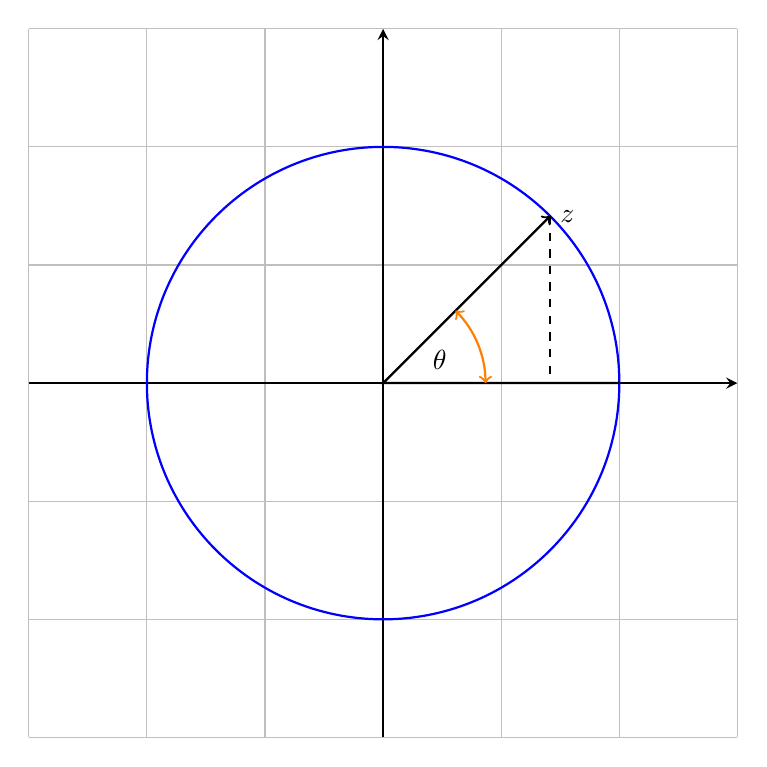
\begin{tikzpicture}
\begin{axis}[
ticks=none,
thick,
x=3cm,
y=3cm,
axis lines=center, 
grid=both,
xmin=-1.5,
xmax=1.5,
ymin=-1.5,
ymax=1.5,
]
\draw[blue, thick] (0,0) circle (1);
\draw[<-] (0.707106781, 0.707106781) coordinate (z) node[right] {$z$}
-- (0,0) coordinate (o) node[right] {}
-- (1,0) coordinate (b) node[right] {}
pic["$\theta$", draw=orange, <->, angle radius=1.3cm]
{angle=b--o--z};
\draw[dashed] (0.707106781, 0.707106781) -- (0.707106781, 0);

\end{axis}
\end{tikzpicture}
\end{center}

\subsection{Quaternions}
Quaternions are very similar to above. If we have some axis $\vec{u}$ we want to rotate about by angle $\theta$, let $\vec{v} = \theta\vec{u}$ be the scaled axis representation of this rotation.
$$q = e^{\theta\vec{u}}$$
$$= 1 - \vec{u}\theta - \frac{\theta^2}{2!} + \frac{\vec{u}\theta^3}{3!} + \dots = \cos\theta + \vec{u}\sin\theta = \begin{bmatrix}
\vec{u}\sin\theta\\
\cos\theta
\end{bmatrix} = \begin{bmatrix}
q_x\\ q_y\\ q_z\\ q_w
\end{bmatrix}$$

\subsubsection{Conjugate}
$$q^* = \begin{bmatrix}
-\vec{u}\sin\theta\\
\cos\theta
\end{bmatrix}$$

\subsubsection{Quaternion Product}
Now we can define the quaternion product:
$$\vec{q} \otimes \vec{p} = [\vec{q}]_l\vec{p} = [\vec{p}]_r\vec{q}$$
$$[\vec{q}]_l = \begin{bmatrix}
q_w & q_z & -q_y & q_x\\
-q_z & q_w & q_x & q_y\\
q_y & -q_x & q_w & q_z\\
-q_x & -q_y & -q_z & q_z 
\end{bmatrix}$$

$$[\vec{q}]_r = \begin{bmatrix}
q_w & -q_z & q_y & q_x\\
q_z & q_w & -q_x & q_y\\
-q_y & q_x & q_w & q_z\\
-q_x & -q_y & -q_z & q_z 
\end{bmatrix}$$

\subsubsection{Rotating a Vector}
We can easily rotate a vector $\vec{x} = \begin{bmatrix}
x_1\\ x_2\\ x_3
\end{bmatrix}$ with quaternion $\vec{q}$. $\vec{q}$ must be a unit vector in order to rotations to be defined.
$$\vec{x}' = \vec{q} \otimes \vec{x} \otimes \vec{q}^* = \vec{q} \otimes \begin{bmatrix}
x_1\\ x_2\\ x_3\\ 0
\end{bmatrix} \otimes \vec{q}^* = [\vec{q}]_l[\vec{q}^*]_r\vec{x} = \begin{bmatrix}
\mat{R} & 0\\
0 & 1
\end{bmatrix}\vec{x}$$ where $\mat{R}$ is a rotation matrix.

It is easiest to construct the rotation matrix as follows:
$$\mat{R} = \begin{bmatrix}
1-2(q_y^2+q_z^2) & 2(q_xq_y-q_zq_w) & 2(q_xq_z+q_yq_w)\\
2(q_xq_y+q_zq_w) & 1 - 2(q_x^2+q_z^2) & 2(q_yq_z-q_xq_w)\\
2(q_xq_z-q_yq_w) & 2(q_yq_z +q_xq_w) & 1-2(q_x^2-q_y^2)
\end{bmatrix}$$
and then $\vec{x}' = \mat{R}\vec{x}$.

\subsection{Why Quaternions?}
You might ask yourself why we should use quaternions over the multitude of other rotation representations? We can list a few of the types here:
\begin{enumerate}
\item Euler angles (roll, pitch, yaw)
\item Scaled axis, like $\theta\vec{u}$ that we constructed our quaternion with
\item Rotation matrix
\end{enumerate}

There are several reasons to use quaternions over these formats and I will list them here:
\begin{enumerate}[(a)]
\item They are free from gimbal lock which Euler angles are perceptable to. This is because quaternions represent a rotation about an axis.
\item The axis angle representation allows us to easily interpolate between orientations or between vectors. Euler angles are noncommutative compositions of rotations about three axes which make it very difficult to interpolate.
\item They only use four variables as opposed to the nine that would be required for a rotation matrix.
\item Unlike the scaled axis representation, we aren't required to do expensive trigonometric computations to construct the rotation matrix.
\end{enumerate}
\end{document}

